


% Header, overrides base

    % Make sure that the sphinx doc style knows who it inherits from.
    \def\sphinxdocclass{article}

    % Declare the document class
    \documentclass[letterpaper,10pt,english]{/Library/Python/2.7/site-packages/Sphinx-1.2-py2.7.egg/sphinx/texinputs/sphinxhowto}

    % Imports
    \usepackage[utf8]{inputenc}
    \DeclareUnicodeCharacter{00A0}{\\nobreakspace}
    \usepackage[T1]{fontenc}
    \usepackage{babel}
    \usepackage{times}
    \usepackage{import}
    \usepackage[Bjarne]{/Library/Python/2.7/site-packages/Sphinx-1.2-py2.7.egg/sphinx/texinputs/fncychap}
    \usepackage{longtable}
    \usepackage{/Library/Python/2.7/site-packages/Sphinx-1.2-py2.7.egg/sphinx/texinputs/sphinx}
    \usepackage{multirow}

    \usepackage{amsmath}
    \usepackage{amssymb}
    \usepackage{ucs}
    \usepackage{enumerate}

    % Used to make the Input/Output rules follow around the contents.
    \usepackage{needspace}

    % Pygments requirements
    \usepackage{fancyvrb}
    \usepackage{color}
    % ansi colors additions
    \definecolor{darkgreen}{rgb}{.12,.54,.11}
    \definecolor{lightgray}{gray}{.95}
    \definecolor{brown}{rgb}{0.54,0.27,0.07}
    \definecolor{purple}{rgb}{0.5,0.0,0.5}
    \definecolor{darkgray}{gray}{0.25}
    \definecolor{lightred}{rgb}{1.0,0.39,0.28}
    \definecolor{lightgreen}{rgb}{0.48,0.99,0.0}
    \definecolor{lightblue}{rgb}{0.53,0.81,0.92}
    \definecolor{lightpurple}{rgb}{0.87,0.63,0.87}
    \definecolor{lightcyan}{rgb}{0.5,1.0,0.83}

    % Needed to box output/input
    \usepackage{tikz}
        \usetikzlibrary{calc,arrows,shadows}
    \usepackage[framemethod=tikz]{mdframed}

    \usepackage{alltt}

    % Used to load and display graphics
    \usepackage{graphicx}
    \graphicspath{ {figs/} }
    \usepackage[Export]{adjustbox} % To resize

    % used so that images for notebooks which have spaces in the name can still be included
    \usepackage{grffile}


    % For formatting output while also word wrapping.
    \usepackage{listings}
    \lstset{breaklines=true}
    \lstset{basicstyle=\small\ttfamily}
    \def\smaller{\fontsize{9.5pt}{9.5pt}\selectfont}

    %Pygments definitions
    
\makeatletter
\def\PY@reset{\let\PY@it=\relax \let\PY@bf=\relax%
    \let\PY@ul=\relax \let\PY@tc=\relax%
    \let\PY@bc=\relax \let\PY@ff=\relax}
\def\PY@tok#1{\csname PY@tok@#1\endcsname}
\def\PY@toks#1+{\ifx\relax#1\empty\else%
    \PY@tok{#1}\expandafter\PY@toks\fi}
\def\PY@do#1{\PY@bc{\PY@tc{\PY@ul{%
    \PY@it{\PY@bf{\PY@ff{#1}}}}}}}
\def\PY#1#2{\PY@reset\PY@toks#1+\relax+\PY@do{#2}}

\expandafter\def\csname PY@tok@gd\endcsname{\def\PY@tc##1{\textcolor[rgb]{0.63,0.00,0.00}{##1}}}
\expandafter\def\csname PY@tok@gu\endcsname{\let\PY@bf=\textbf\def\PY@tc##1{\textcolor[rgb]{0.50,0.00,0.50}{##1}}}
\expandafter\def\csname PY@tok@gt\endcsname{\def\PY@tc##1{\textcolor[rgb]{0.00,0.27,0.87}{##1}}}
\expandafter\def\csname PY@tok@gs\endcsname{\let\PY@bf=\textbf}
\expandafter\def\csname PY@tok@gr\endcsname{\def\PY@tc##1{\textcolor[rgb]{1.00,0.00,0.00}{##1}}}
\expandafter\def\csname PY@tok@cm\endcsname{\let\PY@it=\textit\def\PY@tc##1{\textcolor[rgb]{0.25,0.50,0.50}{##1}}}
\expandafter\def\csname PY@tok@vg\endcsname{\def\PY@tc##1{\textcolor[rgb]{0.10,0.09,0.49}{##1}}}
\expandafter\def\csname PY@tok@m\endcsname{\def\PY@tc##1{\textcolor[rgb]{0.40,0.40,0.40}{##1}}}
\expandafter\def\csname PY@tok@mh\endcsname{\def\PY@tc##1{\textcolor[rgb]{0.40,0.40,0.40}{##1}}}
\expandafter\def\csname PY@tok@go\endcsname{\def\PY@tc##1{\textcolor[rgb]{0.53,0.53,0.53}{##1}}}
\expandafter\def\csname PY@tok@ge\endcsname{\let\PY@it=\textit}
\expandafter\def\csname PY@tok@vc\endcsname{\def\PY@tc##1{\textcolor[rgb]{0.10,0.09,0.49}{##1}}}
\expandafter\def\csname PY@tok@il\endcsname{\def\PY@tc##1{\textcolor[rgb]{0.40,0.40,0.40}{##1}}}
\expandafter\def\csname PY@tok@cs\endcsname{\let\PY@it=\textit\def\PY@tc##1{\textcolor[rgb]{0.25,0.50,0.50}{##1}}}
\expandafter\def\csname PY@tok@cp\endcsname{\def\PY@tc##1{\textcolor[rgb]{0.74,0.48,0.00}{##1}}}
\expandafter\def\csname PY@tok@gi\endcsname{\def\PY@tc##1{\textcolor[rgb]{0.00,0.63,0.00}{##1}}}
\expandafter\def\csname PY@tok@gh\endcsname{\let\PY@bf=\textbf\def\PY@tc##1{\textcolor[rgb]{0.00,0.00,0.50}{##1}}}
\expandafter\def\csname PY@tok@ni\endcsname{\let\PY@bf=\textbf\def\PY@tc##1{\textcolor[rgb]{0.60,0.60,0.60}{##1}}}
\expandafter\def\csname PY@tok@nl\endcsname{\def\PY@tc##1{\textcolor[rgb]{0.63,0.63,0.00}{##1}}}
\expandafter\def\csname PY@tok@nn\endcsname{\let\PY@bf=\textbf\def\PY@tc##1{\textcolor[rgb]{0.00,0.00,1.00}{##1}}}
\expandafter\def\csname PY@tok@no\endcsname{\def\PY@tc##1{\textcolor[rgb]{0.53,0.00,0.00}{##1}}}
\expandafter\def\csname PY@tok@na\endcsname{\def\PY@tc##1{\textcolor[rgb]{0.49,0.56,0.16}{##1}}}
\expandafter\def\csname PY@tok@nb\endcsname{\def\PY@tc##1{\textcolor[rgb]{0.00,0.50,0.00}{##1}}}
\expandafter\def\csname PY@tok@nc\endcsname{\let\PY@bf=\textbf\def\PY@tc##1{\textcolor[rgb]{0.00,0.00,1.00}{##1}}}
\expandafter\def\csname PY@tok@nd\endcsname{\def\PY@tc##1{\textcolor[rgb]{0.67,0.13,1.00}{##1}}}
\expandafter\def\csname PY@tok@ne\endcsname{\let\PY@bf=\textbf\def\PY@tc##1{\textcolor[rgb]{0.82,0.25,0.23}{##1}}}
\expandafter\def\csname PY@tok@nf\endcsname{\def\PY@tc##1{\textcolor[rgb]{0.00,0.00,1.00}{##1}}}
\expandafter\def\csname PY@tok@si\endcsname{\let\PY@bf=\textbf\def\PY@tc##1{\textcolor[rgb]{0.73,0.40,0.53}{##1}}}
\expandafter\def\csname PY@tok@s2\endcsname{\def\PY@tc##1{\textcolor[rgb]{0.73,0.13,0.13}{##1}}}
\expandafter\def\csname PY@tok@vi\endcsname{\def\PY@tc##1{\textcolor[rgb]{0.10,0.09,0.49}{##1}}}
\expandafter\def\csname PY@tok@nt\endcsname{\let\PY@bf=\textbf\def\PY@tc##1{\textcolor[rgb]{0.00,0.50,0.00}{##1}}}
\expandafter\def\csname PY@tok@nv\endcsname{\def\PY@tc##1{\textcolor[rgb]{0.10,0.09,0.49}{##1}}}
\expandafter\def\csname PY@tok@s1\endcsname{\def\PY@tc##1{\textcolor[rgb]{0.73,0.13,0.13}{##1}}}
\expandafter\def\csname PY@tok@sh\endcsname{\def\PY@tc##1{\textcolor[rgb]{0.73,0.13,0.13}{##1}}}
\expandafter\def\csname PY@tok@sc\endcsname{\def\PY@tc##1{\textcolor[rgb]{0.73,0.13,0.13}{##1}}}
\expandafter\def\csname PY@tok@sx\endcsname{\def\PY@tc##1{\textcolor[rgb]{0.00,0.50,0.00}{##1}}}
\expandafter\def\csname PY@tok@bp\endcsname{\def\PY@tc##1{\textcolor[rgb]{0.00,0.50,0.00}{##1}}}
\expandafter\def\csname PY@tok@c1\endcsname{\let\PY@it=\textit\def\PY@tc##1{\textcolor[rgb]{0.25,0.50,0.50}{##1}}}
\expandafter\def\csname PY@tok@kc\endcsname{\let\PY@bf=\textbf\def\PY@tc##1{\textcolor[rgb]{0.00,0.50,0.00}{##1}}}
\expandafter\def\csname PY@tok@c\endcsname{\let\PY@it=\textit\def\PY@tc##1{\textcolor[rgb]{0.25,0.50,0.50}{##1}}}
\expandafter\def\csname PY@tok@mf\endcsname{\def\PY@tc##1{\textcolor[rgb]{0.40,0.40,0.40}{##1}}}
\expandafter\def\csname PY@tok@err\endcsname{\def\PY@bc##1{\setlength{\fboxsep}{0pt}\fcolorbox[rgb]{1.00,0.00,0.00}{1,1,1}{\strut ##1}}}
\expandafter\def\csname PY@tok@kd\endcsname{\let\PY@bf=\textbf\def\PY@tc##1{\textcolor[rgb]{0.00,0.50,0.00}{##1}}}
\expandafter\def\csname PY@tok@ss\endcsname{\def\PY@tc##1{\textcolor[rgb]{0.10,0.09,0.49}{##1}}}
\expandafter\def\csname PY@tok@sr\endcsname{\def\PY@tc##1{\textcolor[rgb]{0.73,0.40,0.53}{##1}}}
\expandafter\def\csname PY@tok@mo\endcsname{\def\PY@tc##1{\textcolor[rgb]{0.40,0.40,0.40}{##1}}}
\expandafter\def\csname PY@tok@kn\endcsname{\let\PY@bf=\textbf\def\PY@tc##1{\textcolor[rgb]{0.00,0.50,0.00}{##1}}}
\expandafter\def\csname PY@tok@mi\endcsname{\def\PY@tc##1{\textcolor[rgb]{0.40,0.40,0.40}{##1}}}
\expandafter\def\csname PY@tok@gp\endcsname{\let\PY@bf=\textbf\def\PY@tc##1{\textcolor[rgb]{0.00,0.00,0.50}{##1}}}
\expandafter\def\csname PY@tok@o\endcsname{\def\PY@tc##1{\textcolor[rgb]{0.40,0.40,0.40}{##1}}}
\expandafter\def\csname PY@tok@kr\endcsname{\let\PY@bf=\textbf\def\PY@tc##1{\textcolor[rgb]{0.00,0.50,0.00}{##1}}}
\expandafter\def\csname PY@tok@s\endcsname{\def\PY@tc##1{\textcolor[rgb]{0.73,0.13,0.13}{##1}}}
\expandafter\def\csname PY@tok@kp\endcsname{\def\PY@tc##1{\textcolor[rgb]{0.00,0.50,0.00}{##1}}}
\expandafter\def\csname PY@tok@w\endcsname{\def\PY@tc##1{\textcolor[rgb]{0.73,0.73,0.73}{##1}}}
\expandafter\def\csname PY@tok@kt\endcsname{\def\PY@tc##1{\textcolor[rgb]{0.69,0.00,0.25}{##1}}}
\expandafter\def\csname PY@tok@ow\endcsname{\let\PY@bf=\textbf\def\PY@tc##1{\textcolor[rgb]{0.67,0.13,1.00}{##1}}}
\expandafter\def\csname PY@tok@sb\endcsname{\def\PY@tc##1{\textcolor[rgb]{0.73,0.13,0.13}{##1}}}
\expandafter\def\csname PY@tok@k\endcsname{\let\PY@bf=\textbf\def\PY@tc##1{\textcolor[rgb]{0.00,0.50,0.00}{##1}}}
\expandafter\def\csname PY@tok@se\endcsname{\let\PY@bf=\textbf\def\PY@tc##1{\textcolor[rgb]{0.73,0.40,0.13}{##1}}}
\expandafter\def\csname PY@tok@sd\endcsname{\let\PY@it=\textit\def\PY@tc##1{\textcolor[rgb]{0.73,0.13,0.13}{##1}}}

\def\PYZbs{\char`\\}
\def\PYZus{\char`\_}
\def\PYZob{\char`\{}
\def\PYZcb{\char`\}}
\def\PYZca{\char`\^}
\def\PYZam{\char`\&}
\def\PYZlt{\char`\<}
\def\PYZgt{\char`\>}
\def\PYZsh{\char`\#}
\def\PYZpc{\char`\%}
\def\PYZdl{\char`\$}
\def\PYZhy{\char`\-}
\def\PYZsq{\char`\'}
\def\PYZdq{\char`\"}
\def\PYZti{\char`\~}
% for compatibility with earlier versions
\def\PYZat{@}
\def\PYZlb{[}
\def\PYZrb{]}
\makeatother


    %Set pygments styles if needed...
    
        \definecolor{nbframe-border}{rgb}{0.867,0.867,0.867}
        \definecolor{nbframe-bg}{rgb}{0.969,0.969,0.969}
        \definecolor{nbframe-in-prompt}{rgb}{0.0,0.0,0.502}
        \definecolor{nbframe-out-prompt}{rgb}{0.545,0.0,0.0}

        \newenvironment{ColorVerbatim}
        {\begin{mdframed}[%
            roundcorner=1.0pt, %
            backgroundcolor=nbframe-bg, %
            userdefinedwidth=1\linewidth, %
            leftmargin=0.1\linewidth, %
            innerleftmargin=0pt, %
            innerrightmargin=0pt, %
            linecolor=nbframe-border, %
            linewidth=1pt, %
            usetwoside=false, %
            everyline=true, %
            innerlinewidth=3pt, %
            innerlinecolor=nbframe-bg, %
            middlelinewidth=1pt, %
            middlelinecolor=nbframe-bg, %
            outerlinewidth=0.5pt, %
            outerlinecolor=nbframe-border, %
            needspace=0pt
        ]}
        {\end{mdframed}}
        
        \newenvironment{InvisibleVerbatim}
        {\begin{mdframed}[leftmargin=0.1\linewidth,innerleftmargin=3pt,innerrightmargin=3pt, userdefinedwidth=1\linewidth, linewidth=0pt, linecolor=white, usetwoside=false]}
        {\end{mdframed}}

        \renewenvironment{Verbatim}[1][\unskip]
        {\begin{alltt}\smaller}
        {\end{alltt}}
    

    % Help prevent overflowing lines due to urls and other hard-to-break 
    % entities.  This doesn't catch everything...
    \sloppy

    % Document level variables
    \title{Math 337 HW02}
    \date{January 31, 2014}
    \release{}
    \author{Andy Reagan}
    \renewcommand{\releasename}{}

    % TODO: Add option for the user to specify a logo for his/her export.
    \newcommand{\sphinxlogo}{}

    % Make the index page of the document.
    \makeindex

    % Import sphinx document type specifics.
     


% Body

    % Start of the document
    \begin{document}

        
            \maketitle
        

        


        
        \section{Problem 1}Derive equation 2.4 following section 1.3\subsubsection*{Solution}From Section 1.4 of the notes we the Taylor expansion of the analytical
solution $y_{i+1}$ as
\[ y_{i+1} = y_i + hf(x_i,y_i) + \frac{h^2}{2} \left ( f_x (x_i,y_i) + f(x_i,y_i)f_y(x_i,y_i) \right ) + O(h^3) .\]
For the general RK form we have the numerical Taylor expansion is
\[ Y_{i+1} = Y_i + (a+b)hf(x_i,Y_i) + bh \left ( \alpha h f_x (x_i,Y_i) + \beta h f(x_i, Y_i) f_y(x_i,Y_i) \right ) + O(h^3) .\]
To find constraints on the coefficients $a,b,\alpha,\beta$ we require
the local error the have $O(h^3)$. Letting $Y_i = y_i$ we solve for the
local error $\epsilon _{i+1} = y_{i+1} - Y_{i+1}$ and set this equal to
the desired $O(h^3)$. This is:

\begin{align*} O(h^3) &= y_i + hf(x_i,y_i) + \frac{h^2}{2} \left ( f_x (x_i,y_i) + f(x_i,y_i)f_y(x_i,y_i) \right ) + O(h^3)\\
&- Y_i - (a+b)hf(x_i,Y_i) - bh \left ( \alpha h f_x (x_i,Y_i) + \beta h f(x_i, Y_i) f_y(x_i,Y_i) \right ) - O(h^3) .\end{align*}

Combining the $O(h^3)$ on the RHS, and subtracting this from both sides,
and letting $Y_i = y_i$, we have

\begin{align*} 0 &= hf(x_i,y_i) + \frac{h^2}{2} f_x (x_i,y_i) + \frac{h^2}{2}f(x_i,y_i)f_y(x_i,y_i) \\
&- (a+b)hf(x_i,y_i) - b  \alpha h^2  f_x (x_i,y_i) - b \beta h^2 f(x_i, y_i) f_y(x_i,y_i).\end{align*}

Grouping terms by the three groups: (1) $f(x_i,y_i)$, (2)
$f_x (x_i,y_i)$, and (3) $f(x_i,y_i) f_y (x_i, y_i)$, we have the three
systems of equations:

\begin{align*} h - (a+b) h &= 0\\
\frac{h^2}{2} - b h^2 \alpha &= 0\\
\frac{h^2}{2} - b h^2 \beta &= 0\end{align*}

Cancelling $h$'s, this is clearly the form of equation 2.4.\section{Problem 2}Write a function implementing the classical runge-kutta scheme, and use
this on problem 5 of the previous HW, plotting the error. Compare the
final error of the cRK method with the ME of the previous HW.\subsubsection*{Solution}The following code solves this problem in Python. For MATLAB, see the
attached printout and emailed file `prb2.m'.

    % Make sure that atleast 4 lines are below the HR
    \needspace{4\baselineskip}

    
        \vspace{6pt}
        \makebox[0.1\linewidth]{\smaller\hfill\tt\color{nbframe-in-prompt}In\hspace{4pt}{[}5{]}:\hspace{4pt}}\\*
        \vspace{-2.65\baselineskip}
        \begin{ColorVerbatim}
            \vspace{-0.7\baselineskip}
            \begin{Verbatim}[commandchars=\\\{\}]
\PY{k+kn}{from} \PY{n+nn}{numpy} \PY{k+kn}{import} \PY{o}{*}

\PY{k}{def} \PY{n+nf}{my\PYZus{}cRK}\PY{p}{(}\PY{n}{func}\PY{p}{,}\PY{n}{tspan}\PY{p}{,}\PY{n}{y0}\PY{p}{,}\PY{n}{h}\PY{p}{,}\PY{n}{params}\PY{p}{)}\PY{p}{:}
    \PY{c}{\PYZsh{} set the coefficients}
    \PY{n}{a11}\PY{p}{,}\PY{n}{a21}\PY{p}{,}\PY{n}{a22}\PY{p}{,}\PY{n}{a31}\PY{p}{,}\PY{n}{a32}\PY{p}{,}\PY{n}{a33} \PY{o}{=} \PY{p}{[}\PY{l+m+mf}{0.5}\PY{p}{,}\PY{l+m+mf}{0.0}\PY{p}{,}\PY{l+m+mf}{0.5}\PY{p}{,}\PY{l+m+mf}{0.0}\PY{p}{,}\PY{l+m+mf}{0.0}\PY{p}{,}\PY{l+m+mf}{1.0}\PY{p}{]}
    \PY{n}{b1}\PY{p}{,}\PY{n}{b2}\PY{p}{,}\PY{n}{b3}\PY{p}{,}\PY{n}{b4} \PY{o}{=} \PY{p}{[}\PY{l+m+mf}{1.}\PY{o}{/}\PY{l+m+mf}{6.}\PY{p}{,}\PY{l+m+mf}{1.}\PY{o}{/}\PY{l+m+mf}{3.}\PY{p}{,}\PY{l+m+mf}{1.}\PY{o}{/}\PY{l+m+mf}{3.}\PY{p}{,}\PY{l+m+mf}{1.}\PY{o}{/}\PY{l+m+mf}{6.}\PY{p}{]}
    \PY{n}{c1}\PY{p}{,}\PY{n}{c2}\PY{p}{,}\PY{n}{c3} \PY{o}{=} \PY{p}{[}\PY{l+m+mf}{0.5}\PY{p}{,}\PY{l+m+mf}{0.5}\PY{p}{,}\PY{l+m+mi}{1}\PY{p}{]}
    \PY{n}{t} \PY{o}{=} \PY{n}{tspan}\PY{p}{[}\PY{l+m+mi}{0}\PY{p}{]}
    
    \PY{n}{yvec} \PY{o}{=}  \PY{p}{[}\PY{p}{]} \PY{c}{\PYZsh{}linspace(tspan[0],tspan[\PYZhy{}1],num=floor((tspan[\PYZhy{}1]\PYZhy{}tspan[0])/h))}
    \PY{n}{yvec}\PY{o}{.}\PY{n}{append}\PY{p}{(}\PY{n}{y0}\PY{p}{)} \PY{c}{\PYZsh{}[0] = y0}
    \PY{k}{for} \PY{n}{i} \PY{o+ow}{in} \PY{n+nb}{xrange}\PY{p}{(}\PY{l+m+mi}{1}\PY{p}{,}\PY{n+nb}{len}\PY{p}{(}\PY{n}{tspan}\PY{p}{)}\PY{p}{)}\PY{p}{:}
        \PY{n}{k1} \PY{o}{=} \PY{n}{h}\PY{o}{*}\PY{n}{func}\PY{p}{(}\PY{n}{t}\PY{p}{,}\PY{n}{yvec}\PY{p}{[}\PY{n}{i}\PY{o}{\PYZhy{}}\PY{l+m+mi}{1}\PY{p}{]}\PY{p}{,}\PY{n}{params}\PY{p}{)}
        \PY{n}{k2} \PY{o}{=} \PY{n}{h}\PY{o}{*}\PY{n}{func}\PY{p}{(}\PY{n}{t}\PY{o}{+}\PY{n}{c1}\PY{o}{*}\PY{n}{h}\PY{p}{,}\PY{n}{yvec}\PY{p}{[}\PY{n}{i}\PY{o}{\PYZhy{}}\PY{l+m+mi}{1}\PY{p}{]}\PY{o}{+}\PY{n}{a11}\PY{o}{*}\PY{n}{k1}\PY{p}{,}\PY{n}{params}\PY{p}{)}
        \PY{n}{k3} \PY{o}{=} \PY{n}{h}\PY{o}{*}\PY{n}{func}\PY{p}{(}\PY{n}{t}\PY{o}{+}\PY{n}{c2}\PY{o}{*}\PY{n}{h}\PY{p}{,}\PY{n}{yvec}\PY{p}{[}\PY{n}{i}\PY{o}{\PYZhy{}}\PY{l+m+mi}{1}\PY{p}{]}\PY{o}{+}\PY{n}{a21}\PY{o}{*}\PY{n}{k1}\PY{o}{+}\PY{n}{a22}\PY{o}{*}\PY{n}{k2}\PY{p}{,}\PY{n}{params}\PY{p}{)}
        \PY{n}{k4} \PY{o}{=} \PY{n}{h}\PY{o}{*}\PY{n}{func}\PY{p}{(}\PY{n}{t}\PY{o}{+}\PY{n}{c3}\PY{o}{*}\PY{n}{h}\PY{p}{,}\PY{n}{yvec}\PY{p}{[}\PY{n}{i}\PY{o}{\PYZhy{}}\PY{l+m+mi}{1}\PY{p}{]}\PY{o}{+}\PY{n}{a31}\PY{o}{*}\PY{n}{k1}\PY{o}{+}\PY{n}{a32}\PY{o}{*}\PY{n}{k2}\PY{o}{+}\PY{n}{a33}\PY{o}{*}\PY{n}{k3}\PY{p}{,}\PY{n}{params}\PY{p}{)}
        \PY{n}{yvec}\PY{o}{.}\PY{n}{append}\PY{p}{(}\PY{n}{yvec}\PY{p}{[}\PY{n}{i}\PY{o}{\PYZhy{}}\PY{l+m+mi}{1}\PY{p}{]} \PY{o}{+} \PY{n}{b1}\PY{o}{*}\PY{n}{k1} \PY{o}{+} \PY{n}{b2}\PY{o}{*}\PY{n}{k2} \PY{o}{+} \PY{n}{b3}\PY{o}{*}\PY{n}{k3} \PY{o}{+} \PY{n}{b4}\PY{o}{*}\PY{n}{k4}\PY{p}{)} \PY{c}{\PYZsh{}[i] = yvec[i\PYZhy{}1] + b1*k1 + b2*k2 + b3*k3 + b4*k4}
        \PY{n}{t} \PY{o}{+}\PY{o}{=} \PY{n}{h}
    \PY{k}{return} \PY{n}{yvec}

\PY{k}{def} \PY{n+nf}{my\PYZus{}ME}\PY{p}{(}\PY{n}{func}\PY{p}{,}\PY{n}{tspan}\PY{p}{,}\PY{n}{y0}\PY{p}{,}\PY{n}{h}\PY{p}{,}\PY{n}{params}\PY{p}{)}\PY{p}{:}
    \PY{n}{yvec} \PY{o}{=} \PY{p}{[}\PY{p}{]}
    \PY{n}{yvec}\PY{o}{.}\PY{n}{append}\PY{p}{(}\PY{n}{y0}\PY{p}{)}
    \PY{n}{t} \PY{o}{=} \PY{n}{tspan}\PY{p}{[}\PY{l+m+mi}{0}\PY{p}{]}
    \PY{k}{for} \PY{n}{i} \PY{o+ow}{in} \PY{n+nb}{xrange}\PY{p}{(}\PY{l+m+mi}{1}\PY{p}{,}\PY{n+nb}{len}\PY{p}{(}\PY{n}{tspan}\PY{p}{)}\PY{p}{)}\PY{p}{:}
        \PY{n}{k1} \PY{o}{=} \PY{n}{func}\PY{p}{(}\PY{n}{t}\PY{p}{,}\PY{n}{yvec}\PY{p}{[}\PY{n}{i}\PY{o}{\PYZhy{}}\PY{l+m+mi}{1}\PY{p}{]}\PY{p}{,}\PY{n}{params}\PY{p}{)}
        \PY{n}{k2} \PY{o}{=} \PY{n}{func}\PY{p}{(}\PY{n}{t}\PY{o}{+}\PY{n}{h}\PY{p}{,}\PY{n}{yvec}\PY{p}{[}\PY{n}{i}\PY{o}{\PYZhy{}}\PY{l+m+mi}{1}\PY{p}{]}\PY{o}{+}\PY{n}{h}\PY{o}{*}\PY{n}{k1}\PY{p}{,}\PY{n}{params}\PY{p}{)}
        \PY{n}{yvec}\PY{o}{.}\PY{n}{append}\PY{p}{(}\PY{n}{yvec}\PY{p}{[}\PY{n}{i}\PY{o}{\PYZhy{}}\PY{l+m+mi}{1}\PY{p}{]}\PY{o}{+}\PY{n}{h}\PY{o}{/}\PY{l+m+mi}{2}\PY{o}{*}\PY{p}{(}\PY{n}{k1}\PY{o}{+}\PY{n}{k2}\PY{p}{)}\PY{p}{)}
        \PY{n}{t}\PY{o}{+}\PY{o}{=}\PY{n}{h}
    \PY{k}{return} \PY{n}{yvec}
\end{Verbatim}

            
                \vspace{-0.2\baselineskip}
            
        \end{ColorVerbatim}
    


    % Make sure that atleast 4 lines are below the HR
    \needspace{4\baselineskip}

    
        \vspace{6pt}
        \makebox[0.1\linewidth]{\smaller\hfill\tt\color{nbframe-in-prompt}In\hspace{4pt}{[}6{]}:\hspace{4pt}}\\*
        \vspace{-2.65\baselineskip}
        \begin{ColorVerbatim}
            \vspace{-0.7\baselineskip}
            \begin{Verbatim}[commandchars=\\\{\}]
\PY{n}{g} \PY{o}{=} \PY{l+m+mf}{9.8}
\PY{n}{k1} \PY{o}{=} \PY{n}{g}\PY{o}{/}\PY{l+m+mf}{35.76} \PY{c}{\PYZsh{} that\PYZsq{}s 80mph in m/s}
\PY{n}{h} \PY{o}{=} \PY{l+m+mf}{0.2}
\PY{n}{y0} \PY{o}{=} \PY{l+m+mf}{0.0}
\PY{n}{x} \PY{o}{=} \PY{n}{linspace}\PY{p}{(}\PY{l+m+mi}{0}\PY{p}{,}\PY{l+m+mi}{2}\PY{p}{,}\PY{n}{num}\PY{o}{=}\PY{n+nb}{int}\PY{p}{(}\PY{l+m+mi}{2}\PY{o}{/}\PY{n}{h}\PY{o}{+}\PY{l+m+mi}{1}\PY{p}{)}\PY{p}{)}
\PY{n}{yAnal} \PY{o}{=} \PY{n}{linspace}\PY{p}{(}\PY{l+m+mi}{0}\PY{p}{,}\PY{l+m+mi}{2}\PY{p}{,}\PY{n}{num}\PY{o}{=}\PY{n+nb}{int}\PY{p}{(}\PY{l+m+mi}{2}\PY{o}{/}\PY{n}{h}\PY{o}{+}\PY{l+m+mi}{1}\PY{p}{)}\PY{p}{)}

\PY{k}{def} \PY{n+nf}{jumperV}\PY{p}{(}\PY{n}{t}\PY{p}{,}\PY{n}{v}\PY{p}{,}\PY{n}{params}\PY{p}{)}\PY{p}{:}
    \PY{c}{\PYZsh{} params = [g,k]}
    \PY{k}{return} \PY{n}{params}\PY{p}{[}\PY{l+m+mi}{0}\PY{p}{]}\PY{o}{\PYZhy{}}\PY{n}{v}\PY{o}{*}\PY{n}{params}\PY{p}{[}\PY{l+m+mi}{1}\PY{p}{]}

\PY{c}{\PYZsh{} use RK4}
\PY{n}{yNumRK4} \PY{o}{=} \PY{n}{my\PYZus{}cRK}\PY{p}{(}\PY{n}{jumperV}\PY{p}{,}\PY{n}{x}\PY{p}{,}\PY{n}{y0}\PY{p}{,}\PY{n}{h}\PY{p}{,}\PY{p}{[}\PY{n}{g}\PY{p}{,}\PY{n}{k1}\PY{p}{]}\PY{p}{)}
\PY{c}{\PYZsh{} solve analytically}
\PY{k}{for} \PY{n}{t} \PY{o+ow}{in} \PY{n+nb}{xrange}\PY{p}{(}\PY{n+nb}{len}\PY{p}{(}\PY{n}{x}\PY{p}{)}\PY{p}{)}\PY{p}{:}
    \PY{n}{yAnal}\PY{p}{[}\PY{n}{t}\PY{p}{]} \PY{o}{=} \PY{o}{\PYZhy{}}\PY{n}{g}\PY{o}{/}\PY{n}{k1}\PY{o}{*}\PY{p}{(}\PY{n}{exp}\PY{p}{(}\PY{o}{\PYZhy{}}\PY{n}{k1}\PY{o}{*}\PY{n}{x}\PY{p}{[}\PY{n}{t}\PY{p}{]}\PY{p}{)}\PY{o}{\PYZhy{}}\PY{l+m+mi}{1}\PY{p}{)}
\PY{c}{\PYZsh{} solve with ME    }
\PY{n}{yNumME} \PY{o}{=} \PY{n}{my\PYZus{}ME}\PY{p}{(}\PY{n}{jumperV}\PY{p}{,}\PY{n}{x}\PY{p}{,}\PY{n}{y0}\PY{p}{,}\PY{n}{h}\PY{p}{,}\PY{p}{[}\PY{n}{g}\PY{p}{,}\PY{n}{k1}\PY{p}{]}\PY{p}{)}
\end{Verbatim}

            
                \vspace{-0.2\baselineskip}
            
        \end{ColorVerbatim}
    


    % Make sure that atleast 4 lines are below the HR
    \needspace{4\baselineskip}

    
        \vspace{6pt}
        \makebox[0.1\linewidth]{\smaller\hfill\tt\color{nbframe-in-prompt}In\hspace{4pt}{[}7{]}:\hspace{4pt}}\\*
        \vspace{-2.65\baselineskip}
        \begin{ColorVerbatim}
            \vspace{-0.7\baselineskip}
            \begin{Verbatim}[commandchars=\\\{\}]
\PY{o}{\PYZpc{}}\PY{k}{matplotlib} \PY{n}{inline}
\PY{k+kn}{import} \PY{n+nn}{matplotlib.pyplot} \PY{k+kn}{as} \PY{n+nn}{plt}
\PY{n}{fig} \PY{o}{=} \PY{n}{plt}\PY{o}{.}\PY{n}{figure}\PY{p}{(}\PY{p}{)}
\PY{n}{ax1} \PY{o}{=} \PY{n}{fig}\PY{o}{.}\PY{n}{add\PYZus{}axes}\PY{p}{(}\PY{p}{[}\PY{l+m+mf}{0.15}\PY{p}{,}\PY{l+m+mf}{0.2}\PY{p}{,}\PY{l+m+mf}{0.7}\PY{p}{,}\PY{l+m+mf}{0.7}\PY{p}{]}\PY{p}{)} \PY{c}{\PYZsh{}  [left, bottom, width, height]  }

\PY{n}{ax1}\PY{o}{.}\PY{n}{plot}\PY{p}{(}\PY{n}{x}\PY{p}{,}\PY{n+nb}{abs}\PY{p}{(}\PY{n}{yAnal}\PY{o}{\PYZhy{}}\PY{n}{yNumRK4}\PY{p}{)}\PY{p}{,}\PY{l+s}{\PYZsq{}}\PY{l+s}{r}\PY{l+s}{\PYZsq{}}\PY{p}{)}
\PY{n}{plt}\PY{o}{.}\PY{n}{title}\PY{p}{(}\PY{l+s}{\PYZsq{}}\PY{l+s}{error of cRK, h = \PYZob{}0:g\PYZcb{}}\PY{l+s}{\PYZsq{}}\PY{o}{.}\PY{n}{format}\PY{p}{(}\PY{n}{h}\PY{p}{)}\PY{p}{)}
\PY{n}{plt}\PY{o}{.}\PY{n}{xlabel}\PY{p}{(}\PY{l+s}{\PYZsq{}}\PY{l+s}{time}\PY{l+s}{\PYZsq{}}\PY{p}{)}
\PY{n}{plt}\PY{o}{.}\PY{n}{ylabel}\PY{p}{(}\PY{l+s}{\PYZsq{}}\PY{l+s}{magnitude of error}\PY{l+s}{\PYZsq{}}\PY{p}{)}
\PY{n}{plt}\PY{o}{.}\PY{n}{show}\PY{p}{(}\PY{p}{)}

\PY{n}{plt}\PY{o}{.}\PY{n}{close}\PY{p}{(}\PY{n}{fig}\PY{p}{)}
\end{Verbatim}

            
                \vspace{-0.2\baselineskip}
            
        \end{ColorVerbatim}
    

    

        % If the first block is an image, minipage the image.  Else
        % request a certain amount of space for the input text.
        \needspace{4\baselineskip}
        
        

            % Add document contents.
            
                \begin{InvisibleVerbatim}
                \vspace{-0.5\baselineskip}
    \begin{center}
    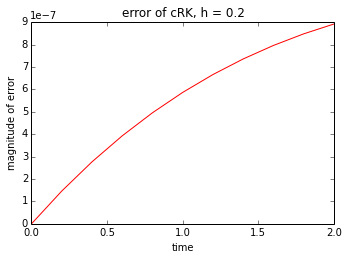
\includegraphics[max size={\textwidth}{\textheight}]{hw02_files/hw02_10_0.png}
    \par
    \end{center}
    
            \end{InvisibleVerbatim}
            
        
    


    % Make sure that atleast 4 lines are below the HR
    \needspace{4\baselineskip}

    
        \vspace{6pt}
        \makebox[0.1\linewidth]{\smaller\hfill\tt\color{nbframe-in-prompt}In\hspace{4pt}{[}8{]}:\hspace{4pt}}\\*
        \vspace{-2.65\baselineskip}
        \begin{ColorVerbatim}
            \vspace{-0.7\baselineskip}
            \begin{Verbatim}[commandchars=\\\{\}]
\PY{n}{error\PYZus{}ME} \PY{o}{=} \PY{n}{yAnal}\PY{p}{[}\PY{o}{\PYZhy{}}\PY{l+m+mi}{1}\PY{p}{]}\PY{o}{\PYZhy{}}\PY{n}{yNumME}\PY{p}{[}\PY{o}{\PYZhy{}}\PY{l+m+mi}{1}\PY{p}{]}
\PY{n}{error\PYZus{}RK4} \PY{o}{=} \PY{n}{yAnal}\PY{p}{[}\PY{o}{\PYZhy{}}\PY{l+m+mi}{1}\PY{p}{]}\PY{o}{\PYZhy{}}\PY{n}{yNumRK4}\PY{p}{[}\PY{o}{\PYZhy{}}\PY{l+m+mi}{1}\PY{p}{]}
\PY{k}{print} \PY{l+s}{\PYZsq{}}\PY{l+s}{final error of ME is \PYZob{}0:.9f\PYZcb{}}\PY{l+s}{\PYZsq{}}\PY{o}{.}\PY{n}{format}\PY{p}{(}\PY{n}{error\PYZus{}ME}\PY{p}{)}
\PY{k}{print} \PY{l+s}{\PYZsq{}}\PY{l+s}{final error of cRK is \PYZob{}0:.9f\PYZcb{}}\PY{l+s}{\PYZsq{}}\PY{o}{.}\PY{n}{format}\PY{p}{(}\PY{n}{error\PYZus{}RK4}\PY{p}{)}
\PY{k}{print}
\PY{k}{print} \PY{l+s}{\PYZsq{}}\PY{l+s}{ratio of cRK/ME is \PYZob{}0:.5f\PYZcb{}}\PY{l+s}{\PYZsq{}}\PY{o}{.}\PY{n}{format}\PY{p}{(}\PY{n}{error\PYZus{}RK4}\PY{o}{/}\PY{n}{error\PYZus{}ME}\PY{p}{)}
\PY{k}{print} \PY{n}{h}\PY{o}{*}\PY{o}{*}\PY{l+m+mi}{2}
\PY{k}{print} \PY{n}{h}\PY{o}{*}\PY{o}{*}\PY{l+m+mi}{4}
\end{Verbatim}

            
                \vspace{-0.2\baselineskip}
            
        \end{ColorVerbatim}
    

    

        % If the first block is an image, minipage the image.  Else
        % request a certain amount of space for the input text.
        \needspace{4\baselineskip}
        
        

            % Add document contents.
            
                \begin{InvisibleVerbatim}
                \vspace{-0.5\baselineskip}
\begin{alltt}final error of ME is 0.005911787
final error of cRK is 0.000000892

ratio of cRK/ME is 0.00015
0.04
0.0016
\end{alltt}

            \end{InvisibleVerbatim}
            
        
    
\section{Problem 3}Open the parachute at time $t=2$, with new velocity being 4 mph.\subsubsection*{Solution}Again, the following inline solution uses some Python. The attached
MALTAB script `prb3.m' implements this.

The new coefficient $k$ is:

    % Make sure that atleast 4 lines are below the HR
    \needspace{4\baselineskip}

    
        \vspace{6pt}
        \makebox[0.1\linewidth]{\smaller\hfill\tt\color{nbframe-in-prompt}In\hspace{4pt}{[}9{]}:\hspace{4pt}}\\*
        \vspace{-2.65\baselineskip}
        \begin{ColorVerbatim}
            \vspace{-0.7\baselineskip}
            \begin{Verbatim}[commandchars=\\\{\}]
\PY{n}{k2} \PY{o}{=} \PY{n}{g}\PY{o}{/}\PY{l+m+mf}{1.788}
\PY{k}{print} \PY{n}{k2}
\end{Verbatim}

            
                \vspace{-0.2\baselineskip}
            
        \end{ColorVerbatim}
    

    

        % If the first block is an image, minipage the image.  Else
        % request a certain amount of space for the input text.
        \needspace{4\baselineskip}
        
        

            % Add document contents.
            
                \begin{InvisibleVerbatim}
                \vspace{-0.5\baselineskip}
\begin{alltt}5.48098434004
\end{alltt}

            \end{InvisibleVerbatim}
            
        
    
Define a new function for the ODE:

    % Make sure that atleast 4 lines are below the HR
    \needspace{4\baselineskip}

    
        \vspace{6pt}
        \makebox[0.1\linewidth]{\smaller\hfill\tt\color{nbframe-in-prompt}In\hspace{4pt}{[}10{]}:\hspace{4pt}}\\*
        \vspace{-2.65\baselineskip}
        \begin{ColorVerbatim}
            \vspace{-0.7\baselineskip}
            \begin{Verbatim}[commandchars=\\\{\}]
\PY{k}{def} \PY{n+nf}{jumperV2}\PY{p}{(}\PY{n}{t}\PY{p}{,}\PY{n}{v}\PY{p}{,}\PY{n}{params}\PY{p}{)}\PY{p}{:}
    \PY{c}{\PYZsh{} params = [g,k1,k2]}
    \PY{k}{if} \PY{n}{t}\PY{o}{\PYZlt{}}\PY{l+m+mi}{2}\PY{p}{:}
        \PY{k}{return} \PY{n}{params}\PY{p}{[}\PY{l+m+mi}{0}\PY{p}{]}\PY{o}{\PYZhy{}}\PY{n}{v}\PY{o}{*}\PY{n}{params}\PY{p}{[}\PY{l+m+mi}{1}\PY{p}{]}
    \PY{k}{else}\PY{p}{:}
        \PY{k}{return} \PY{n}{params}\PY{p}{[}\PY{l+m+mi}{0}\PY{p}{]}\PY{o}{\PYZhy{}}\PY{n}{v}\PY{o}{*}\PY{n}{params}\PY{p}{[}\PY{l+m+mi}{2}\PY{p}{]}
\end{Verbatim}

            
                \vspace{-0.2\baselineskip}
            
        \end{ColorVerbatim}
    
The new analytical solution for the ODE is the same, but with a
different $k$ and hence a different $y0$. Now I'll make a quick plot of
that solution (using a finer $h$ to see the behavior):

    % Make sure that atleast 4 lines are below the HR
    \needspace{4\baselineskip}

    
        \vspace{6pt}
        \makebox[0.1\linewidth]{\smaller\hfill\tt\color{nbframe-in-prompt}In\hspace{4pt}{[}11{]}:\hspace{4pt}}\\*
        \vspace{-2.65\baselineskip}
        \begin{ColorVerbatim}
            \vspace{-0.7\baselineskip}
            \begin{Verbatim}[commandchars=\\\{\}]
\PY{n}{x} \PY{o}{=} \PY{n}{linspace}\PY{p}{(}\PY{l+m+mi}{0}\PY{p}{,}\PY{l+m+mi}{4}\PY{p}{,}\PY{n}{num}\PY{o}{=}\PY{l+m+mi}{21}\PY{p}{)} \PY{c}{\PYZsh{}int(4/h+1))}
\PY{n}{yAnal} \PY{o}{=} \PY{n}{linspace}\PY{p}{(}\PY{l+m+mi}{0}\PY{p}{,}\PY{l+m+mi}{4}\PY{p}{,}\PY{n}{num}\PY{o}{=}\PY{l+m+mi}{21}\PY{p}{)} \PY{c}{\PYZsh{}int(4/h+1))}
\PY{k}{print} \PY{n}{k2}\PY{o}{/}\PY{n}{k1}
\PY{k}{print} \PY{n}{g} \PY{o}{\PYZhy{}} \PY{n}{k2}\PY{o}{*}\PY{n}{g}\PY{o}{/}\PY{n}{k1}\PY{o}{*}\PY{p}{(}\PY{o}{\PYZhy{}}\PY{n}{exp}\PY{p}{(}\PY{o}{\PYZhy{}}\PY{n}{k1}\PY{o}{*}\PY{l+m+mi}{2}\PY{p}{)}\PY{o}{+}\PY{l+m+mi}{1}\PY{p}{)}

\PY{c}{\PYZsh{} solve analytically}
\PY{k}{for} \PY{n}{i} \PY{o+ow}{in} \PY{n+nb}{xrange}\PY{p}{(}\PY{n+nb}{len}\PY{p}{(}\PY{n}{x}\PY{p}{)}\PY{p}{)}\PY{p}{:}
    \PY{n}{t} \PY{o}{=} \PY{n}{x}\PY{p}{[}\PY{n}{i}\PY{p}{]}
    \PY{k}{if} \PY{n}{t}\PY{o}{\PYZlt{}}\PY{l+m+mi}{2}\PY{p}{:}
        \PY{n}{yAnal}\PY{p}{[}\PY{n}{i}\PY{p}{]} \PY{o}{=} \PY{o}{\PYZhy{}}\PY{n}{g}\PY{o}{/}\PY{n}{k1}\PY{o}{*}\PY{p}{(}\PY{n}{exp}\PY{p}{(}\PY{o}{\PYZhy{}}\PY{n}{k1}\PY{o}{*}\PY{n}{t}\PY{p}{)}\PY{o}{\PYZhy{}}\PY{l+m+mi}{1}\PY{p}{)}
    \PY{k}{else}\PY{p}{:}
        \PY{n}{yAnal}\PY{p}{[}\PY{n}{i}\PY{p}{]} \PY{o}{=} \PY{p}{(}\PY{o}{\PYZhy{}}\PY{n}{exp}\PY{p}{(}\PY{o}{\PYZhy{}}\PY{n}{k2}\PY{o}{*}\PY{p}{(}\PY{n}{t}\PY{o}{\PYZhy{}}\PY{l+m+mi}{2}\PY{p}{)}\PY{p}{)}\PY{o}{*}\PY{p}{(}\PY{n}{k2}\PY{o}{/}\PY{n}{k1}\PY{o}{*}\PY{n}{exp}\PY{p}{(}\PY{o}{\PYZhy{}}\PY{l+m+mi}{2}\PY{o}{*}\PY{n}{k1}\PY{p}{)}\PY{o}{\PYZhy{}}\PY{n}{k2}\PY{o}{/}\PY{n}{k1}\PY{o}{+}\PY{l+m+mi}{1}\PY{p}{)}\PY{o}{+}\PY{l+m+mi}{1}\PY{p}{)}\PY{o}{*}\PY{n}{g}\PY{o}{/}\PY{n}{k2}

\PY{n}{yNumRK4} \PY{o}{=} \PY{n}{my\PYZus{}cRK}\PY{p}{(}\PY{n}{jumperV2}\PY{p}{,}\PY{n}{x}\PY{p}{,}\PY{n}{y0}\PY{p}{,}\PY{n}{h}\PY{p}{,}\PY{p}{[}\PY{n}{g}\PY{p}{,}\PY{n}{k1}\PY{p}{,}\PY{n}{k2}\PY{p}{]}\PY{p}{)}
\PY{n}{yNumME} \PY{o}{=} \PY{n}{my\PYZus{}ME}\PY{p}{(}\PY{n}{jumperV2}\PY{p}{,}\PY{n}{x}\PY{p}{,}\PY{n}{y0}\PY{p}{,}\PY{n}{h}\PY{p}{,}\PY{p}{[}\PY{n}{g}\PY{p}{,}\PY{n}{k1}\PY{p}{,}\PY{n}{k2}\PY{p}{]}\PY{p}{)}

\PY{n}{fig} \PY{o}{=} \PY{n}{plt}\PY{o}{.}\PY{n}{figure}\PY{p}{(}\PY{p}{)}
\PY{n}{ax1} \PY{o}{=} \PY{n}{fig}\PY{o}{.}\PY{n}{add\PYZus{}axes}\PY{p}{(}\PY{p}{[}\PY{l+m+mf}{0.15}\PY{p}{,}\PY{l+m+mf}{0.2}\PY{p}{,}\PY{l+m+mf}{0.7}\PY{p}{,}\PY{l+m+mf}{0.7}\PY{p}{]}\PY{p}{)} \PY{c}{\PYZsh{}  [left, bottom, width, height]  }

\PY{n}{ax1}\PY{o}{.}\PY{n}{plot}\PY{p}{(}\PY{n}{x}\PY{p}{,}\PY{n}{yAnal}\PY{p}{,}\PY{l+s}{\PYZsq{}}\PY{l+s}{r}\PY{l+s}{\PYZsq{}}\PY{p}{)}
\PY{n}{ax1}\PY{o}{.}\PY{n}{plot}\PY{p}{(}\PY{n}{x}\PY{p}{,}\PY{n}{yNumRK4}\PY{p}{,}\PY{l+s}{\PYZsq{}}\PY{l+s}{b}\PY{l+s}{\PYZsq{}}\PY{p}{)}
\PY{n}{ax1}\PY{o}{.}\PY{n}{plot}\PY{p}{(}\PY{n}{x}\PY{p}{,}\PY{n}{yNumME}\PY{p}{,}\PY{l+s}{\PYZsq{}}\PY{l+s}{c}\PY{l+s}{\PYZsq{}}\PY{p}{)}
\PY{n}{plt}\PY{o}{.}\PY{n}{legend}\PY{p}{(}\PY{p}{[}\PY{l+s}{\PYZdq{}}\PY{l+s}{analytical}\PY{l+s}{\PYZdq{}}\PY{p}{,}\PY{l+s}{\PYZdq{}}\PY{l+s}{RK4}\PY{l+s}{\PYZdq{}}\PY{p}{,}\PY{l+s}{\PYZdq{}}\PY{l+s}{ME}\PY{l+s}{\PYZdq{}}\PY{p}{]}\PY{p}{)}
\PY{n}{plt}\PY{o}{.}\PY{n}{show}\PY{p}{(}\PY{p}{)}
\PY{n}{plt}\PY{o}{.}\PY{n}{close}\PY{p}{(}\PY{n}{fig}\PY{p}{)}
\end{Verbatim}

            
                \vspace{-0.2\baselineskip}
            
        \end{ColorVerbatim}
    

    

        % If the first block is an image, minipage the image.  Else
        % request a certain amount of space for the input text.
        \needspace{4\baselineskip}
        
        

            % Add document contents.
            
                \begin{InvisibleVerbatim}
                \vspace{-0.5\baselineskip}
\begin{alltt}20.0
-72.9025993903
\end{alltt}

            \end{InvisibleVerbatim}
            
                \begin{InvisibleVerbatim}
                \vspace{-0.5\baselineskip}
    \begin{center}
    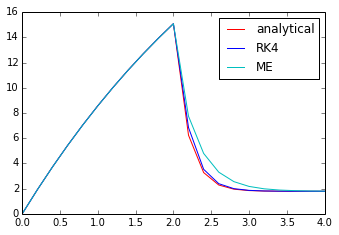
\includegraphics[max size={\textwidth}{\textheight}]{hw02_files/hw02_20_1.png}
    \par
    \end{center}
    
            \end{InvisibleVerbatim}
            
        
    
\section{Problem 4}Code RKF and solve the above using it.

The matlab script `my\_RKF.m' implements this function in MATLAB, and
the following is reproduced in `prb4.m'.\subsubsection*{Solution}

    % Make sure that atleast 4 lines are below the HR
    \needspace{4\baselineskip}

    
        \vspace{6pt}
        \makebox[0.1\linewidth]{\smaller\hfill\tt\color{nbframe-in-prompt}In\hspace{4pt}{[}14{]}:\hspace{4pt}}\\*
        \vspace{-2.65\baselineskip}
        \begin{ColorVerbatim}
            \vspace{-0.7\baselineskip}
            \begin{Verbatim}[commandchars=\\\{\}]
\PY{k}{def} \PY{n+nf}{my\PYZus{}RKF}\PY{p}{(}\PY{n}{func}\PY{p}{,}\PY{n}{tspan}\PY{p}{,}\PY{n}{y0}\PY{p}{,}\PY{n}{h}\PY{p}{,}\PY{n}{params}\PY{p}{)}\PY{p}{:}
    \PY{n}{max\PYZus{}error} \PY{o}{=} \PY{l+m+mi}{10}\PY{o}{*}\PY{o}{*}\PY{p}{(}\PY{o}{\PYZhy{}}\PY{l+m+mi}{1}\PY{p}{)}\PY{o}{*}\PY{l+m+mf}{0.44704} \PY{c}{\PYZsh{} 10\PYZca{}\PYZhy{}3 mph in m/s}
    \PY{n}{kappa} \PY{o}{=} \PY{l+m+mf}{0.8}
    \PY{c}{\PYZsh{} accept the tspan, but use only the range of it}
    \PY{n}{t} \PY{o}{=} \PY{n}{tspan}\PY{p}{[}\PY{l+m+mi}{0}\PY{p}{]}
    \PY{c}{\PYZsh{} accept h, use it for the first guess}
    \PY{n}{newh} \PY{o}{=} \PY{n}{h}
    \PY{c}{\PYZsh{} t \PYZhy{}= newH}
    \PY{c}{\PYZsh{} set the coefficients}
    \PY{n}{a11} \PY{o}{=} \PY{l+m+mf}{0.25}
    \PY{n}{a21}\PY{p}{,}\PY{n}{a22} \PY{o}{=} \PY{p}{[}\PY{l+m+mf}{3.}\PY{o}{/}\PY{l+m+mf}{32.}\PY{p}{,}\PY{l+m+mf}{9.}\PY{o}{/}\PY{l+m+mf}{32.}\PY{p}{]}
    \PY{n}{a31}\PY{p}{,}\PY{n}{a32}\PY{p}{,}\PY{n}{a33} \PY{o}{=} \PY{p}{[}\PY{l+m+mf}{1932.}\PY{o}{/}\PY{l+m+mf}{2197.}\PY{p}{,}\PY{o}{\PYZhy{}}\PY{l+m+mf}{7200.}\PY{o}{/}\PY{l+m+mf}{2197.}\PY{p}{,}\PY{l+m+mf}{7296.}\PY{o}{/}\PY{l+m+mf}{2197.}\PY{p}{]}
    \PY{n}{a41}\PY{p}{,}\PY{n}{a42}\PY{p}{,}\PY{n}{a43}\PY{p}{,}\PY{n}{a44} \PY{o}{=} \PY{p}{[}\PY{l+m+mf}{439.}\PY{o}{/}\PY{l+m+mf}{216.}\PY{p}{,}\PY{o}{\PYZhy{}}\PY{l+m+mf}{8.}\PY{p}{,}\PY{l+m+mf}{3680.}\PY{o}{/}\PY{l+m+mf}{513.}\PY{p}{,}\PY{o}{\PYZhy{}}\PY{l+m+mf}{845.}\PY{o}{/}\PY{l+m+mf}{4104.}\PY{p}{]}
    \PY{n}{a51}\PY{p}{,}\PY{n}{a52}\PY{p}{,}\PY{n}{a53}\PY{p}{,}\PY{n}{a54}\PY{p}{,}\PY{n}{a55} \PY{o}{=} \PY{p}{[}\PY{o}{\PYZhy{}}\PY{l+m+mf}{8.}\PY{o}{/}\PY{l+m+mf}{27.}\PY{p}{,}\PY{l+m+mf}{2.0}\PY{p}{,}\PY{o}{\PYZhy{}}\PY{l+m+mf}{3544.}\PY{o}{/}\PY{l+m+mf}{2565.}\PY{p}{,}\PY{l+m+mf}{1859.}\PY{o}{/}\PY{l+m+mf}{4104.}\PY{p}{,}\PY{o}{\PYZhy{}}\PY{l+m+mf}{11.}\PY{o}{/}\PY{l+m+mf}{40.}\PY{p}{]}
    \PY{n}{b41}\PY{p}{,}\PY{n}{b42}\PY{p}{,}\PY{n}{b43}\PY{p}{,}\PY{n}{b44}\PY{p}{,}\PY{n}{b45}\PY{p}{,}\PY{n}{b46} \PY{o}{=} \PY{p}{[}\PY{l+m+mf}{25.}\PY{o}{/}\PY{l+m+mi}{216}\PY{p}{,}\PY{l+m+mf}{0.0}\PY{p}{,}\PY{l+m+mf}{1408.}\PY{o}{/}\PY{l+m+mf}{2565.}\PY{p}{,}\PY{l+m+mf}{2197.}\PY{o}{/}\PY{l+m+mf}{4104.}\PY{p}{,}\PY{o}{\PYZhy{}}\PY{l+m+mf}{1.}\PY{o}{/}\PY{l+m+mf}{5.}\PY{p}{,}\PY{l+m+mf}{0.0}\PY{p}{]}
    \PY{n}{b51}\PY{p}{,}\PY{n}{b52}\PY{p}{,}\PY{n}{b53}\PY{p}{,}\PY{n}{b54}\PY{p}{,}\PY{n}{b55}\PY{p}{,}\PY{n}{b56} \PY{o}{=} \PY{p}{[}\PY{l+m+mf}{16.}\PY{o}{/}\PY{l+m+mf}{135.}\PY{p}{,}\PY{l+m+mf}{0.0}\PY{p}{,}\PY{l+m+mf}{6656.}\PY{o}{/}\PY{l+m+mf}{12825.}\PY{p}{,}\PY{l+m+mf}{28561.}\PY{o}{/}\PY{l+m+mf}{56430.}\PY{p}{,}\PY{o}{\PYZhy{}}\PY{l+m+mf}{9.}\PY{o}{/}\PY{l+m+mf}{50.}\PY{p}{,}\PY{l+m+mf}{2.}\PY{o}{/}\PY{l+m+mf}{55.}\PY{p}{]}
    \PY{n}{c1}\PY{p}{,}\PY{n}{c2}\PY{p}{,}\PY{n}{c3}\PY{p}{,}\PY{n}{c4}\PY{p}{,}\PY{n}{c5} \PY{o}{=} \PY{p}{[}\PY{l+m+mf}{0.25}\PY{p}{,}\PY{l+m+mf}{3.}\PY{o}{/}\PY{l+m+mf}{8.}\PY{p}{,}\PY{l+m+mf}{12.}\PY{o}{/}\PY{l+m+mf}{13.}\PY{p}{,}\PY{l+m+mf}{1.0}\PY{p}{,}\PY{l+m+mf}{0.5}\PY{p}{]}
    \PY{n}{yvec} \PY{o}{=}  \PY{p}{[}\PY{p}{]} \PY{c}{\PYZsh{}linspace(tspan[0],tspan[\PYZhy{}1],num=floor((tspan[\PYZhy{}1]\PYZhy{}tspan[0])/h))}
    \PY{n}{yvec}\PY{o}{.}\PY{n}{append}\PY{p}{(}\PY{n}{y0}\PY{p}{)} \PY{c}{\PYZsh{}[0] = y0}
    \PY{n}{tvec} \PY{o}{=}  \PY{p}{[}\PY{p}{]} \PY{c}{\PYZsh{}linspace(tspan[0],tspan[\PYZhy{}1],num=floor((tspan[\PYZhy{}1]\PYZhy{}tspan[0])/h))}
    \PY{n}{tvec}\PY{o}{.}\PY{n}{append}\PY{p}{(}\PY{n}{t}\PY{p}{)} \PY{c}{\PYZsh{}[0] = y0}
    
    \PY{c}{\PYZsh{} for i in xrange(1,len(tspan)):}
    \PY{k}{while} \PY{n}{t}\PY{o}{\PYZlt{}}\PY{n}{tspan}\PY{p}{[}\PY{o}{\PYZhy{}}\PY{l+m+mi}{1}\PY{p}{]}\PY{p}{:}

        
        \PY{n}{k1} \PY{o}{=} \PY{n}{newh}\PY{o}{*}\PY{n}{func}\PY{p}{(}\PY{n}{t}\PY{p}{,}\PY{n}{yvec}\PY{p}{[}\PY{o}{\PYZhy{}}\PY{l+m+mi}{1}\PY{p}{]}\PY{p}{,}\PY{n}{params}\PY{p}{)}
        \PY{n}{k2} \PY{o}{=} \PY{n}{newh}\PY{o}{*}\PY{n}{func}\PY{p}{(}\PY{n}{t}\PY{o}{+}\PY{n}{c1}\PY{o}{*}\PY{n}{newh}\PY{p}{,}\PY{n}{yvec}\PY{p}{[}\PY{o}{\PYZhy{}}\PY{l+m+mi}{1}\PY{p}{]}\PY{o}{+}\PY{n}{a11}\PY{o}{*}\PY{n}{k1}\PY{p}{,}\PY{n}{params}\PY{p}{)}
        \PY{n}{k3} \PY{o}{=} \PY{n}{newh}\PY{o}{*}\PY{n}{func}\PY{p}{(}\PY{n}{t}\PY{o}{+}\PY{n}{c2}\PY{o}{*}\PY{n}{newh}\PY{p}{,}\PY{n}{yvec}\PY{p}{[}\PY{o}{\PYZhy{}}\PY{l+m+mi}{1}\PY{p}{]}\PY{o}{+}\PY{n}{a21}\PY{o}{*}\PY{n}{k1}\PY{o}{+}\PY{n}{a22}\PY{o}{*}\PY{n}{k2}\PY{p}{,}\PY{n}{params}\PY{p}{)}
        \PY{n}{k4} \PY{o}{=} \PY{n}{newh}\PY{o}{*}\PY{n}{func}\PY{p}{(}\PY{n}{t}\PY{o}{+}\PY{n}{c3}\PY{o}{*}\PY{n}{newh}\PY{p}{,}\PY{n}{yvec}\PY{p}{[}\PY{o}{\PYZhy{}}\PY{l+m+mi}{1}\PY{p}{]}\PY{o}{+}\PY{n}{a31}\PY{o}{*}\PY{n}{k1}\PY{o}{+}\PY{n}{a32}\PY{o}{*}\PY{n}{k2}\PY{o}{+}\PY{n}{a33}\PY{o}{*}\PY{n}{k3}\PY{p}{,}\PY{n}{params}\PY{p}{)}
        \PY{n}{k5} \PY{o}{=} \PY{n}{newh}\PY{o}{*}\PY{n}{func}\PY{p}{(}\PY{n}{t}\PY{o}{+}\PY{n}{c4}\PY{o}{*}\PY{n}{newh}\PY{p}{,}\PY{n}{yvec}\PY{p}{[}\PY{o}{\PYZhy{}}\PY{l+m+mi}{1}\PY{p}{]}\PY{o}{+}\PY{n}{a41}\PY{o}{*}\PY{n}{k1}\PY{o}{+}\PY{n}{a42}\PY{o}{*}\PY{n}{k2}\PY{o}{+}\PY{n}{a43}\PY{o}{*}\PY{n}{k3}\PY{o}{+}\PY{n}{a44}\PY{o}{*}\PY{n}{k4}\PY{p}{,}\PY{n}{params}\PY{p}{)}
        \PY{n}{k6} \PY{o}{=} \PY{n}{newh}\PY{o}{*}\PY{n}{func}\PY{p}{(}\PY{n}{t}\PY{o}{+}\PY{n}{c5}\PY{o}{*}\PY{n}{newh}\PY{p}{,}\PY{n}{yvec}\PY{p}{[}\PY{o}{\PYZhy{}}\PY{l+m+mi}{1}\PY{p}{]}\PY{o}{+}\PY{n}{a51}\PY{o}{*}\PY{n}{k1}\PY{o}{+}\PY{n}{a52}\PY{o}{*}\PY{n}{k2}\PY{o}{+}\PY{n}{a53}\PY{o}{*}\PY{n}{k3}\PY{o}{+}\PY{n}{a54}\PY{o}{*}\PY{n}{k4}\PY{o}{+}\PY{n}{a55}\PY{o}{*}\PY{n}{k5}\PY{p}{,}\PY{n}{params}\PY{p}{)}
        \PY{n}{y4} \PY{o}{=} \PY{n}{yvec}\PY{p}{[}\PY{o}{\PYZhy{}}\PY{l+m+mi}{1}\PY{p}{]} \PY{o}{+} \PY{n}{b41}\PY{o}{*}\PY{n}{k1} \PY{o}{+} \PY{n}{b42}\PY{o}{*}\PY{n}{k2} \PY{o}{+} \PY{n}{b43}\PY{o}{*}\PY{n}{k3} \PY{o}{+} \PY{n}{b44}\PY{o}{*}\PY{n}{k4} \PY{o}{+} \PY{n}{b45}\PY{o}{*}\PY{n}{k5} \PY{o}{+} \PY{n}{b46}\PY{o}{*}\PY{n}{k6}
        \PY{n}{y5} \PY{o}{=} \PY{n}{yvec}\PY{p}{[}\PY{o}{\PYZhy{}}\PY{l+m+mi}{1}\PY{p}{]} \PY{o}{+} \PY{n}{b51}\PY{o}{*}\PY{n}{k1} \PY{o}{+} \PY{n}{b52}\PY{o}{*}\PY{n}{k2} \PY{o}{+} \PY{n}{b53}\PY{o}{*}\PY{n}{k3} \PY{o}{+} \PY{n}{b54}\PY{o}{*}\PY{n}{k4} \PY{o}{+} \PY{n}{b55}\PY{o}{*}\PY{n}{k5} \PY{o}{+} \PY{n}{b56}\PY{o}{*}\PY{n}{k6}
        
        \PY{n}{error\PYZus{}guess} \PY{o}{=} \PY{n+nb}{abs}\PY{p}{(}\PY{n}{y5}\PY{o}{\PYZhy{}}\PY{n}{y4}\PY{p}{)}
        \PY{k}{if} \PY{n}{error\PYZus{}guess} \PY{o}{\PYZlt{}} \PY{n}{max\PYZus{}error}\PY{p}{:}
            \PY{n}{t} \PY{o}{+}\PY{o}{=} \PY{n}{newh}
            \PY{n}{tvec}\PY{o}{.}\PY{n}{append}\PY{p}{(}\PY{n}{t}\PY{p}{)}
            \PY{n}{yvec}\PY{o}{.}\PY{n}{append}\PY{p}{(}\PY{n}{y5}\PY{p}{)}
        \PY{k}{else}\PY{p}{:}
            \PY{k}{if} \PY{n}{newh} \PY{o}{\PYZlt{}} \PY{l+m+mi}{10}\PY{o}{*}\PY{o}{*}\PY{p}{(}\PY{o}{\PYZhy{}}\PY{l+m+mi}{5}\PY{p}{)}\PY{p}{:}
                \PY{n}{tvec}\PY{o}{.}\PY{n}{append}\PY{p}{(}\PY{n}{t}\PY{p}{)}
                \PY{n}{yvec}\PY{o}{.}\PY{n}{append}\PY{p}{(}\PY{n}{y5}\PY{p}{)}
            \PY{k}{else}\PY{p}{:}
                \PY{n}{newh} \PY{o}{=} \PY{n}{newh}\PY{o}{*}\PY{n}{kappa}\PY{o}{*}\PY{p}{(}\PY{p}{(}\PY{n}{max\PYZus{}error}\PY{o}{/}\PY{n}{error\PYZus{}guess}\PY{p}{)}\PY{o}{*}\PY{o}{*}\PY{p}{(}\PY{l+m+mi}{1}\PY{o}{/}\PY{p}{(}\PY{l+m+mi}{4}\PY{o}{+}\PY{l+m+mi}{1}\PY{p}{)}\PY{p}{)}\PY{p}{)}

    \PY{k}{return} \PY{n}{yvec}\PY{p}{,}\PY{n}{tvec}
\end{Verbatim}

            
                \vspace{-0.2\baselineskip}
            
        \end{ColorVerbatim}
    


    % Make sure that atleast 4 lines are below the HR
    \needspace{4\baselineskip}

    
        \vspace{6pt}
        \makebox[0.1\linewidth]{\smaller\hfill\tt\color{nbframe-in-prompt}In\hspace{4pt}{[}15{]}:\hspace{4pt}}\\*
        \vspace{-2.65\baselineskip}
        \begin{ColorVerbatim}
            \vspace{-0.7\baselineskip}
            \begin{Verbatim}[commandchars=\\\{\}]
\PY{n}{yNumRKF}\PY{p}{,}\PY{n}{tNumRKF} \PY{o}{=} \PY{n}{my\PYZus{}RKF}\PY{p}{(}\PY{n}{jumperV2}\PY{p}{,}\PY{n}{x}\PY{p}{,}\PY{n}{y0}\PY{p}{,}\PY{n}{h}\PY{p}{,}\PY{p}{[}\PY{n}{g}\PY{p}{,}\PY{n}{k1}\PY{p}{,}\PY{n}{k2}\PY{p}{]}\PY{p}{)}


\PY{c}{\PYZsh{} solve analytically on new time grid}
\PY{n}{yAnal} \PY{o}{=} \PY{p}{[}\PY{p}{]}
\PY{k}{for} \PY{n}{i} \PY{o+ow}{in} \PY{n+nb}{xrange}\PY{p}{(}\PY{n+nb}{len}\PY{p}{(}\PY{n}{tNumRKF}\PY{p}{)}\PY{p}{)}\PY{p}{:}
    \PY{n}{t} \PY{o}{=} \PY{n}{tNumRKF}\PY{p}{[}\PY{n}{i}\PY{p}{]}
    \PY{k}{if} \PY{n}{t}\PY{o}{\PYZlt{}}\PY{l+m+mi}{2}\PY{p}{:}
        \PY{n}{yAnal}\PY{o}{.}\PY{n}{append}\PY{p}{(}\PY{o}{\PYZhy{}}\PY{n}{g}\PY{o}{/}\PY{n}{k1}\PY{o}{*}\PY{p}{(}\PY{n}{exp}\PY{p}{(}\PY{o}{\PYZhy{}}\PY{n}{k1}\PY{o}{*}\PY{n}{t}\PY{p}{)}\PY{o}{\PYZhy{}}\PY{l+m+mi}{1}\PY{p}{)}\PY{p}{)}
    \PY{k}{else}\PY{p}{:}
        \PY{n}{yAnal}\PY{o}{.}\PY{n}{append}\PY{p}{(}\PY{p}{(}\PY{o}{\PYZhy{}}\PY{n}{exp}\PY{p}{(}\PY{o}{\PYZhy{}}\PY{n}{k2}\PY{o}{*}\PY{p}{(}\PY{n}{t}\PY{o}{\PYZhy{}}\PY{l+m+mi}{2}\PY{p}{)}\PY{p}{)}\PY{o}{*}\PY{p}{(}\PY{n}{k2}\PY{o}{/}\PY{n}{k1}\PY{o}{*}\PY{n}{exp}\PY{p}{(}\PY{o}{\PYZhy{}}\PY{l+m+mi}{2}\PY{o}{*}\PY{n}{k1}\PY{p}{)}\PY{o}{\PYZhy{}}\PY{n}{k2}\PY{o}{/}\PY{n}{k1}\PY{o}{+}\PY{l+m+mi}{1}\PY{p}{)}\PY{o}{+}\PY{l+m+mi}{1}\PY{p}{)}\PY{o}{*}\PY{n}{g}\PY{o}{/}\PY{n}{k2}\PY{p}{)}

\PY{n}{fig} \PY{o}{=} \PY{n}{plt}\PY{o}{.}\PY{n}{figure}\PY{p}{(}\PY{p}{)}
\PY{n}{ax1} \PY{o}{=} \PY{n}{fig}\PY{o}{.}\PY{n}{add\PYZus{}axes}\PY{p}{(}\PY{p}{[}\PY{l+m+mf}{0.15}\PY{p}{,}\PY{l+m+mf}{0.2}\PY{p}{,}\PY{l+m+mf}{0.7}\PY{p}{,}\PY{l+m+mf}{0.7}\PY{p}{]}\PY{p}{)} \PY{c}{\PYZsh{}  [left, bottom, width, height]  }

\PY{n}{ax1}\PY{o}{.}\PY{n}{plot}\PY{p}{(}\PY{n}{tNumRKF}\PY{p}{,}\PY{n}{yAnal}\PY{p}{,}\PY{l+s}{\PYZsq{}}\PY{l+s}{r}\PY{l+s}{\PYZsq{}}\PY{p}{)}
\PY{n}{ax1}\PY{o}{.}\PY{n}{plot}\PY{p}{(}\PY{n}{tNumRKF}\PY{p}{,}\PY{n}{yNumRKF}\PY{p}{,}\PY{l+s}{\PYZsq{}}\PY{l+s}{b}\PY{l+s}{\PYZsq{}}\PY{p}{)}
\PY{n}{plt}\PY{o}{.}\PY{n}{legend}\PY{p}{(}\PY{p}{[}\PY{l+s}{\PYZdq{}}\PY{l+s}{analytical}\PY{l+s}{\PYZdq{}}\PY{p}{,}\PY{l+s}{\PYZdq{}}\PY{l+s}{RKF}\PY{l+s}{\PYZdq{}}\PY{p}{]}\PY{p}{)}
\PY{n}{plt}\PY{o}{.}\PY{n}{show}\PY{p}{(}\PY{p}{)}
\PY{n}{plt}\PY{o}{.}\PY{n}{close}\PY{p}{(}\PY{n}{fig}\PY{p}{)}
\end{Verbatim}

            
                \vspace{-0.2\baselineskip}
            
        \end{ColorVerbatim}
    

    

        % If the first block is an image, minipage the image.  Else
        % request a certain amount of space for the input text.
        \needspace{4\baselineskip}
        
        

            % Add document contents.
            
                \begin{InvisibleVerbatim}
                \vspace{-0.5\baselineskip}
    \begin{center}
    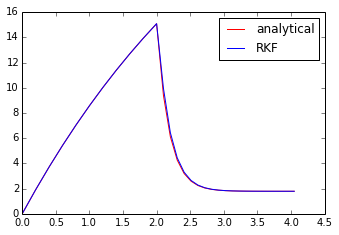
\includegraphics[max size={\textwidth}{\textheight}]{hw02_files/hw02_25_0.png}
    \par
    \end{center}
    
            \end{InvisibleVerbatim}
            
        
    


    % Make sure that atleast 4 lines are below the HR
    \needspace{4\baselineskip}

    
        \vspace{6pt}
        \makebox[0.1\linewidth]{\smaller\hfill\tt\color{nbframe-in-prompt}In\hspace{4pt}{[}37{]}:\hspace{4pt}}\\*
        \vspace{-2.65\baselineskip}
        \begin{ColorVerbatim}
            \vspace{-0.7\baselineskip}
            \begin{Verbatim}[commandchars=\\\{\}]
\PY{n}{tNumRKF}\PY{p}{[}\PY{l+m+mi}{0}\PY{p}{]}
\end{Verbatim}

            
                \vspace{-0.2\baselineskip}
            
        \end{ColorVerbatim}
    

    

        % If the first block is an image, minipage the image.  Else
        % request a certain amount of space for the input text.
        \needspace{4\baselineskip}
        
        

            % Add document contents.
            
                \makebox[0.1\linewidth]{\smaller\hfill\tt\color{nbframe-out-prompt}Out\hspace{4pt}{[}37{]}:\hspace{4pt}}\\*
                \vspace{-2.55\baselineskip}\begin{InvisibleVerbatim}
                \vspace{-0.5\baselineskip}
\begin{alltt}-0.20000000000000001\end{alltt}

            \end{InvisibleVerbatim}
            
        
    
\section{Problem 5}Solve problem 3 using MATLAB's built in ode45. Plot the analytical and
numerical solution.\subsubsection*{Solution}The solution was run in MATLAB and saved as a CSV. We load it and make
the plots.

    % Make sure that atleast 4 lines are below the HR
    \needspace{4\baselineskip}

    
        \vspace{6pt}
        \makebox[0.1\linewidth]{\smaller\hfill\tt\color{nbframe-in-prompt}In\hspace{4pt}{[}18{]}:\hspace{4pt}}\\*
        \vspace{-2.65\baselineskip}
        \begin{ColorVerbatim}
            \vspace{-0.7\baselineskip}
            \begin{Verbatim}[commandchars=\\\{\}]
\PY{o}{!}!/Applications/MATLAB\PYZus{}R2013a.app/bin/matlab \PYZhy{}nodesktop \PYZhy{}nosplash \PYZhy{}r /Users/andyreagan/class/2014/fall/math337/hw02/prb5.m
\end{Verbatim}

            
                \vspace{-0.2\baselineskip}
            
        \end{ColorVerbatim}
    

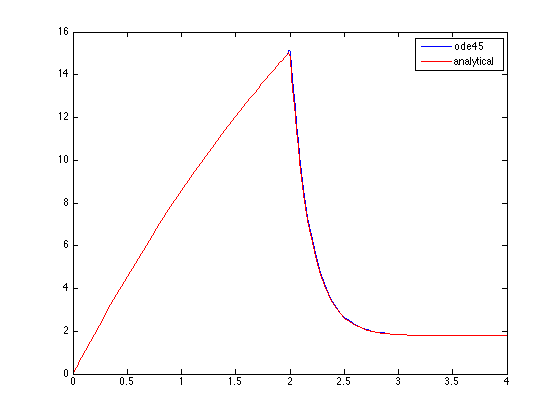
\includegraphics[width=300px]{prb5.png}
        
    
\section{Problem 6}Plot all of the errors on the same plot (3-5)\subsubsection*{Solution}If the previous MATLAB scripts, prb{[}3-5{]}.m, have been executed, then
prb6.m makes this plot. Otherwise, run those script to load the errors
in the local namespace.

    % Make sure that atleast 4 lines are below the HR
    \needspace{4\baselineskip}

    
        \vspace{6pt}
        \makebox[0.1\linewidth]{\smaller\hfill\tt\color{nbframe-in-prompt}In\hspace{4pt}{[}68{]}:\hspace{4pt}}\\*
        \vspace{-2.65\baselineskip}
        \begin{ColorVerbatim}
            \vspace{-0.7\baselineskip}
            \begin{Verbatim}[commandchars=\\\{\}]
\PY{o}{!}!matlab \PYZhy{}r prb6.m
\end{Verbatim}

            
                \vspace{-0.2\baselineskip}
            
        \end{ColorVerbatim}
    
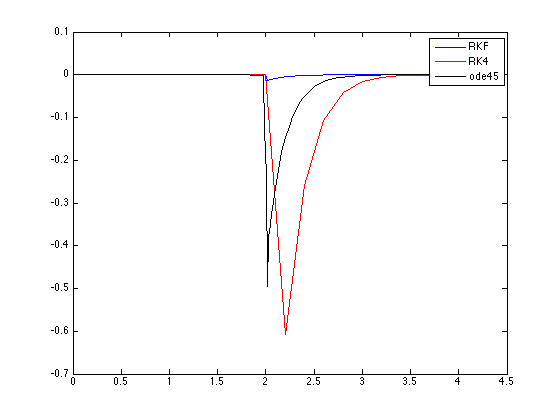
\includegraphics[width=300px]{prb6.png}

        

        \renewcommand{\indexname}{Index}
        \printindex

    % End of document
    \end{document}


